\section{Construction}
To fill in the rest, we need to construct addition, multiplication, negation and inversion of constructable numbers.
In the followuing chapter the proof shema is given by construct lines and such that the wanted point is there intersection. Thefore aren't in the handout just the constructionn.
The full proofs can be would in the Blueprint.

\begin{lemma}[Addition of complex numbers]
    \label{lem:construction_add}
    For $z_1, z_2 \in M_{\infty}$ is $z_1 + z_2 \in M_{\infty}$.
\end{lemma}
This constrution is teken from \cite{JAN_SCHROEER:2023}.\\
One can construct the point $z_1 + z_2$ by drawing a circle with center $z_1$ and radius $\|z_2\|$ and a circle with center $z_2$ and radius $\|z_1\|$ and taking the intersection of the two circles.\ref{Fig.2}

\begin{figure}[h!]
    \centering
    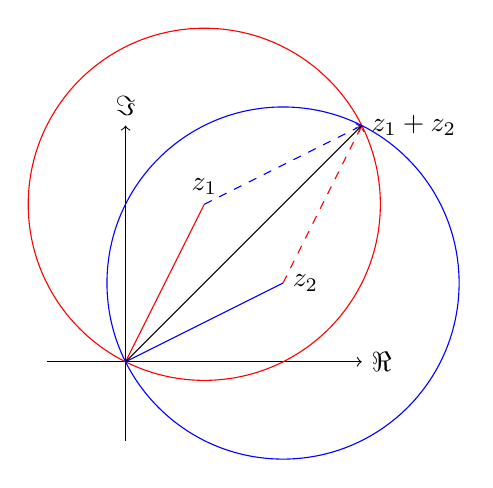
\begin{tikzpicture}
        \draw[->] (-1,0) -- (3,0) node[right] {$\Re$};
        \draw[->] (0,-1) -- (0,3) node[above] {$\Im$};
        \draw (0,0) -- (1,2) node[above] {$z_1$}[red];
        \draw (0,0) -- (2,1) node[right] {$z_2$}[blue];
        \draw (1,2) circle (2.2360679775)[red];
        \draw (2,1) circle (2.2360679775)[blue];
        \draw[dashed,->] (1,2) -- (3,3)[blue];
        \draw[dashed,->] (2,1) -- (3,3)[red];
        \draw (0,0) -- (3,3) node[right] {$z_1 + z_2$};
    \end{tikzpicture}
    \caption{Construction of $z_1 + z_2$}
    \label{Fig.2}
\end{figure}

\begin{lstlisting}
    lemma add_M_Inf (M: Set ℂ) (h₀: (0:ℂ)∈ M) (z₁ z₂ : ℂ) (hz₁ : z₁ ∈ (M_inf M)) (hz₂ : z₂ ∈ (M_inf M)):
            z₁ + z₂ ∈ (M_inf M) := by
        let c₁ : Construction.circle := {c := z₁, r := (dist 0 z₂)}
        let c₂ : Construction.circle := {c := z₂, r := (dist 0 z₁)}
        have hc₁ : c₁ ∈ C (M_inf M) := by
            use z₁, 0, z₂
            refine ⟨?_, (by exact hz₁), (by exact M_M_inf M h₀), (by exact hz₂)⟩
            simp [c₁]
        have hc₂ : c₂ ∈ C (M_inf M) := by
            use z₂, 0, z₁
            refine ⟨?_, (by exact hz₂), (by exact M_M_inf M h₀), (by exact hz₁)⟩
            simp [c₂]
        apply icc_M_inf M
        refine ⟨c₁, (by exact hc₁), c₂, (by exact hc₂), ?_⟩
        simp [circle.points, Set.mem_inter_iff]
\end{lstlisting}

\begin{lemma}[Negative complex numbers]
    \label{lem:construction_neg}
    \lean{z_neg_M_inf}
    \leanok
    \uses{def:set_of_constructable_points}
    For $z \in M_{\infty}$ is $-z \in M_{\infty}$.
\end{lemma}
This constrution is teken from \cite{JAN_SCHROEER:2023}.\\
To get the point $-z$ we can use the second intersection of the line through $0$ and $z$ with circle with center $0$ and radius $\|z\|$.\ref{Fig.1}

\begin{figure}[h!]
    \centering
    \begin{tikzpicture}
        \draw[->] (-1,0) -- (3,0) node[right] {$\Re$};
        \draw[->] (0,-1) -- (0,3) node[above] {$\Im$};
        \draw (0,0) -- (2,2) node[right] {$z$};
        \draw (0,0) -- (-2,-2) node[left] {$-z$};
        \draw (0,0) circle (2.8);
    \end{tikzpicture}
    \caption{Construction of $-z$}
    \label{Fig.1}
\end{figure}

\begin{lstlisting}
    lemma z_neg_M_inf (M: Set ℂ) (h₀: (0:ℂ)∈ M) (z : ℂ) (hz : z ∈ (M_inf M)) : -z ∈ (M_inf M) := by
        by_cases z0:(z=0)
        . simp [z0, M_M_inf M h₀]
        let l : line := {z₁ := 0, z₂ := z}
        let c : Construction.circle := {c := 0, r := (dist 0 z)}
        have hl : l ∈ L (M_inf M) := by
            use 0, z
            refine ⟨?_, (by apply M_M_inf M h₀), (by exact hz), ?_⟩
            simp only [l]
            simp  [eq_comm, z0]
        have hc : c ∈ C (M_inf M) := by
            use 0, 0, z
            refine ⟨?_, (by exact M_M_inf M h₀), (by exact M_M_inf M h₀), (by exact hz)⟩
            simp [l, c]
        apply ilc_M_inf M
        refine ⟨c , (by exact hc), l, (by exact hl), ?_⟩
        simp [circle.points, line.points]
        use 2
        push_cast
        ring_nf
\end{lstlisting}

\begin{lemma}[Multiplication of positve real numbers]
    \label{lem:construction_mul}
    \lean{ab_in_M_inf}
    \leanok
    \uses{def:set_of_constructable_points}
    For $a, b \in M_{\infty}\cap\R$ is $a \cdot b \in M_{\infty}$.
\end{lemma}
This constrution is taken from \cite{cox2012galois}.\\
To get the point $a\cdot b$ we draw a line trough $a$ and $\imath$ and a parallel line through $\imath b$. The intersection of the second line with the real axis is $a\cdot b$.\ref{Fig.5} 

\begin{figure}[h!]
    \centering
    \begin{tikzpicture}
        \draw[->] (-0.5,0) -- (5,0) node[right] {$\Re$};
        \draw[->] (0,-0.5) -- (0,3) node[above] {$\Im$};
        \coordinate[label=135:$\imath$] (i) at (0,1);
        \coordinate[label=-90:$a$] (a) at (2,0);
        \coordinate[label=135:$\imath b$] (ib) at (0,2);
        \coordinate[label=-90:$ab$] (ab) at (4,0);
        \fill[black] (i) circle (2pt);
        \fill[black] (a) circle (2pt);
        \fill[black] (ib) circle (2pt);
        \fill[black] (ab) circle (2pt);
        \draw (a) -- (i);
        \draw (ib) -- (ab);
    \end{tikzpicture}
    \caption{Construction of $z_1 \cdot z_2$}
    \label{Fig.5}
\end{figure}

\begin{corollary}[Multiplication of complex numbers]
    \label{cor:construction_mul_complex}
    %\lean{mul_in_M_inf}
    %\leanok
    \uses{def:set_of_constructable_points}
    For $z_1, z_2 \in M_{\infty}$ is $z_1 \cdot z_2$ in $M_{\infty}$.
\end{corollary}
\begin{proof}
    \uses{lem:construction_mul, lem:construction_add, cor:construction_sub, lem:construction_real, lem:construction_imag}
    Let $z_1 = a + \imath b$ and $z_2 = c + \imath d$. Then $$z_1 \cdot z_2 = (a + \imath b) \cdot (c + \imath d) = (a \cdot c - b \cdot d) + \imath (a \cdot d + b \cdot c).$$
    By combeing the Lemmas \ref{lem:construction_mul}, \ref{lem:construction_add}, \ref{cor:construction_sub}, \ref{lem:construction_real} and \ref{lem:construction_imag} we get that $z_1 \cdot z_2 \in M_{\infty}$.
\end{proof}


\begin{lemma}[Invers of a pos real number]
    \label{lem:construction_inv}
    \lean{ainv_in_M_inf}
    \leanok
    \uses{def:set_of_constructable_points}
    If $a \in M_{\infty}\cap\R$, then $a^{-1}$ is in  $M_{\infty}$.
\end{lemma}

This can be construceted analog to the multiplication of positve real numbers. Usind the fact that $a\cdot a^{-1} = 1$. Draw a line through $1$ and $\imath a$ and a parallel line through $\imath$. The intersection of the second line with the real axis is $a^{-1}$.\ref{Fig.6}
\begin{proof}
    \uses{def:line, def:set_of_lines, lem:ill_M_inf, lem:construction_imath_r, cor:construction_imath, lem:construction_add, cor:construction_sub}
    The proof is analog to the proof of Lemma \ref{lem:construction_mul} we just need two lines $l = \{1-\imath z + \imath, \imath\}$ and $l_{\Re} = \{1,0\}$.\\
    With  out loss of generality we can assume that $a \ne 0$.\\
    That there are in $\mathcal{L(M_{\infty})}$ follows analog to the proof of Lemma \ref{lem:construction_mul}.\\ 
    So we have just to show that $z^{-1} \in l$, i.e. $\exists t: t  (1 - \imath a + \imath) + (1 - t)  I = a^{-1}$ $$t  (1 - \imath a + \imath) + (1 - t)  \imath \stackrel{t:=a^{-1}}{=}  a^{-1} - a^{-1} \imath a + a^{-1}\imath + \imath - a^{-1}\imath = a^{-1}.$$
    The rest follws analog.
\end{proof}
\begin{figure}[h!]
    \centering
    \begin{tikzpicture}
        \draw[->] (-1,0) -- (2,0) node[right] {$\Re$};
        \draw[->] (0,-1) -- (0,3) node[above] {$\Im$};
        \coordinate[label=135:$\imath$] (i) at (0,1);
        \coordinate[label=-90:$1$] (1) at (1,0);
        \coordinate[label=135:$\imath a$] (ia) at (0,2);
        \coordinate[label=-90:$a^{-1}$] (ainv) at (0.5,0);
        \fill[black] (i) circle (2pt);
        \fill[black] (1) circle (2pt);
        \fill[black] (ia) circle (2pt);
        \fill[black] (ainv) circle (2pt);
        \draw (1) -- (ia);
        \draw (i) -- (ainv);
    \end{tikzpicture}
    \caption{Construction of $z^{-1}$}
    \label{Fig.6}
\end{figure}

\begin{corollary}[Invers of a complex number]
    \label{cor:inv_M_inf}
    \lean{inv_M_inf, z_inv_eq}
    \leanok
    \uses{def:set_of_constructable_points}
    If $z \in M_{\infty}$, then $z^{-1}$ is in  $M_{\infty}$.
\end{corollary}
\begin{proof}
    \uses{lem:construction_inv, lem:construction_mul, cor:construction_sub, lem:construction_real, lem:construction_imag, lem:construction_add}
    For $z \in M_{\infty}$ we can write $z = a + \imath b$ with $a, b \in \R$. Then
    $$z^{-1} = \frac{1}{z} = \frac{\overline{z}}{z\overline{z}} = \frac{a - \imath b}{a^2+b^2}= (a - \imath b) \cdot (aa+bb)^{-1}.$$
    Now we can again combiened the lemmas for addition\ref{lem:construction_add}, subtraction\ref{cor:construction_sub}, multiplication\ref{cor:construction_mul_complex} and the corollary for the invers of a positive real number\ref{lem:construction_inv} with the exists of real an imaginary\ref{construction_re_im} part to get that $z^{-1} \in M_{\infty}$.
\end{proof}